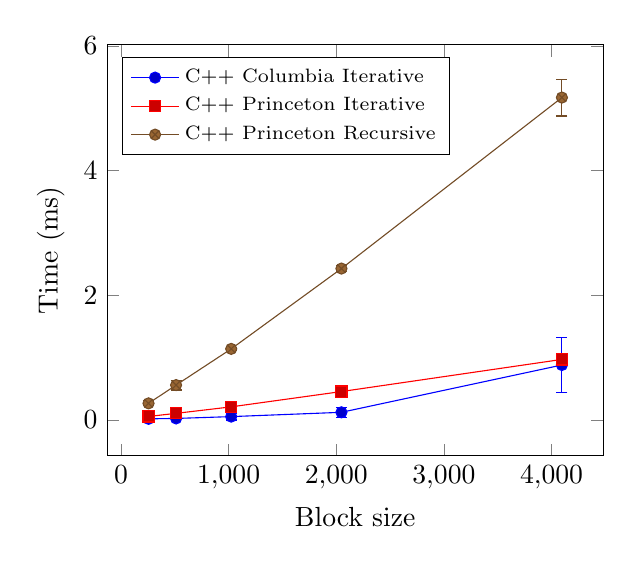
\begin{tikzpicture}
\begin{axis}[xlabel={Block size},ylabel={Time (ms)},width=0.65\linewidth,legend pos=north west,scaled y ticks = false,legend cell align=left,legend style={font=\scriptsize}]
\addplot+[error bars/.cd, y dir=both,y explicit] coordinates {
(256, 0.0160) +- (0.0408, 0.0408)
(512, 0.0223) +- (0.0032, 0.0032)
(1024, 0.0516) +- (0.0547, 0.0547)
(2048, 0.1206) +- (0.0787, 0.0787)
(4096, 0.8794) +- (0.4366, 0.4366)
};
\addplot+[error bars/.cd, y dir=both,y explicit] coordinates {
(256, 0.0541) +- (0.0048, 0.0048)
(512, 0.1038) +- (0.0056, 0.0056)
(1024, 0.2082) +- (0.0127, 0.0127)
(2048, 0.4536) +- (0.0536, 0.0536)
(4096, 0.9690) +- (0.0314, 0.0314)
};
\addplot+[error bars/.cd, y dir=both,y explicit] coordinates {
(256, 0.2642) +- (0.0405, 0.0405)
(512, 0.5573) +- (0.0791, 0.0791)
(1024, 1.1380) +- (0.0245, 0.0245)
(2048, 2.4265) +- (0.0476, 0.0476)
(4096, 5.1699) +- (0.2963, 0.2963)
};
\legend{C++ Columbia Iterative , C++ Princeton Iterative , C++ Princeton Recursive}
\end{axis}
\end{tikzpicture}
